\documentclass[12pt,a4paper]{article}
\usepackage[utf8]{inputenc}
\usepackage{amsmath}
\usepackage{amsfonts}
\usepackage{amssymb}
\usepackage{graphicx}
\usepackage{booktabs}
\usepackage{natbib}
\usepackage{dcolumn}
\usepackage{setspace}
\usepackage{array}
\usepackage{pdflscape} %allows for rotating pages with wide tables
\newcolumntype{P}[1]{>{\raggedright\arraybackslash}p{#1}}
%\usepackage{tabulary}
\usepackage[T1]{fontenc}
\usepackage{lmodern}
\usepackage{multirow}
\usepackage{multicol}

%\usepackage{mathptmx} %times font
%\usepackage{tgtermes} %times font
\usepackage[protrusion=true,expansion=true]{microtype}
\usepackage[top=1in, bottom=1in, left=1in, right=1in]{geometry}
\usepackage{hyperref}
\usepackage{color,soul} %highlighting
\usepackage{caption}
\captionsetup[figure]{labelfont=bf}
\captionsetup[table]{labelfont=bf}

%\usepackage{endnotes}
%\usepackage[heads,nolists,tablesfirst]{endfloat} %places tables and figures at the end
%



\usepackage{epstopdf}

\title{\textbf{Housing Bubbles and \\Support for Governing Parties}}


\author{
Frederik Hjorth \and Martin V. Larsen}

%, \textt{fh@ifs.ku.dk}, (+45) 26 27 24 41 }  } 


\begin{document}

\maketitle

\begin{center}
\textsc{draft - please do not quote, cite, or circulate}
\end{center}

\begin{abstract}
\noindent When the real estate bubble burst in 2007 it had profound consequences for the state of the world economy. However, we know little about whether or how this housing bubble affected voting behavior. Studying the electoral consequences is important, because it helps us understand how voters react to economic shocks which affect their immediate environment and, in turn, the incentives reelection-minded politicians face when trying to deal with economic bubbles. In this paper, we zoom in on one country, Denmark, a country which had exceptionally volatile house prices, and examine how this rapid expansion and contraction of real estate prices shaped support for governing parties across four parliamentary elections. To do this, we link detailed data on local house prices to election returns at the precinct level. Across a wide range of demanding specifications, we find that the when house prices change so does the governing parties vote share. Further, this relationship seems to be stronger in areas where house prices are very volatile, and when the change in house prices are negative.
 
\end{abstract}

%\begin{keyword}
%\doublespacing
%%x \sep y
%\end{keyword}

%\end{frontmatter}

\newpage

%\onehalfspacing
\doublespacing

\section{Introduction}
In this article we examine how local house prices shaped the electoral success of governing parties in Danish parliamentary elections from 2005 till 2015. A period in which the real-estate market in Denmark experienced a dramatic boom and bust \citep{dam2011housing}. Specifically, we want to examine whether voters held governing politicians electorally accountable, in the sense of electorally punishing and rewarding them, for changes in house-prices in their community. That is, whether a decline in house prices in a community means that voters in this community are less likely to support governing parties. 

Compared to other features of the economy, the quality and status of one's home has recieved scant attention in extant literature on economic voting. A small literature exists on patrimonial economic voting \citep{nadeau2010patrimonial,stubager2013reaching}, that is the extent to which owning assets, like real estate, makes it more likely that you will vote for right-wing parties \citep[see][for a similar argument]{ansell2014political}. However, very few studies and have focused on whether house prices, similarly to other economic indicators like unemployment and GDP per capita, influence electoral support for governing parties. Further, in the few studies which do include house prices, their effects are rarely examined in detail \citep[e.g.,][]{hopkins2015economic}. 

Understanding how the housing bubble affected support for governing parties is important for at least two reasons. First of all, just like we can learn about political business cycles from studying voter myopia \citep{healy2014substituting,tufte1980political}, or learn about the prevalence of disaster relief vis-à-vis disaster prevention by looking at how voters reward spending on one or the other \citep{healy2009myopic,ashworth2012electoral}, studying how voters react to housing bubbles tells us something about the political antecedents of these bubbles. Specifically, it highlights the incentives reelection-minded politicians face when developing policies which influence the formation of economic bubbles.

Second of all, studying house prices allows us to understand how local economic conditions shape electoral support for governing politicians. Something which is interesting in light of the fact that most studies of the electoral effects of the economy has focused on the national economy or, to a lesser extent, personal economic conditions \citep[290]{healy2013retrospective}. To the extent that we find that voters do hold politicians accountable for economic conditions in the local context, this means that politicians cannot simply be attentive to economic conditions as a whole, but has to worry about the geographic distribution of these conditions \citep[cf.][11]{ferejohn1986incumbent}. 

A number of existing studies have examined the political effects played by local economic conditions. A set of studies have looked at whether local economic conditions affect voters' perceptions of the national economy; they generally find mixed or small effects (\citealt{books1999contextual,reeves2012ecologies,anderson2011local,ansolabehere2014mecro}, though see \citealt{dinesen2015reconsidering}). Another set of studies have looked at consequences for support for governing parties, finding mixed or statistically insignificant effects of local economic conditions \citep{hansford2015reevaluating,eisenberg2004economic,kim2003spatial}. As such, the existing literature has not been able to show strong effects of local economic conditions. This might mean that they are not at all important for voters. However, it might also mean that previous literature has simply been unable to identify these effects. There are some issues with the data and methods used in previous research, which suggest that the latter might be true.

First, previous literature have  generally relied on rather large geographical units (e.g. US counties) when estimating the effects of local economic conditions. This is potentially problematic, as the local context voters react to, might not map on to these large geographical areas. Second, the studies do not generally take structural differences between local contexts into account when relating economic conditions to  attitudes or voting behavior. This is potentially problematic, since it seems likely that voters will at least take some structural factors into account. In the present case, voters are probably not likely to infer much about the government based on the fact that there are differences in house prices between cities and rural areas. They are more likely to infer based on the fact that their house prices are declining, or that they are not rising less than they usually do. Related to this, one risks conflating re-distributive concerns, i.e. voters in comparatively less well off areas having different demands from government than those in well of areas, with inferential concerns, what does my local context tell me about the national economy or about the quality of the government. Third, the measures of local economic conditions are often based on samples which, while large enough to estimate precise national economic conditions, are not sufficiently precise on geographical levels. Taken together, these factors make it likely that previous studies do not estimate an reasonably efficient estimate of the effect of local economic conditions. 

In the present study we address all of these shortcomings by (1) using data on a small geographical level of aggregation (precincts), (2) using panel data which removes influence from context-specific and time-invariant confounders, and (3) using detailed register data on all real estate transactions in the period under investigation. 

Analyzing these data, we find that changes in house prices do lead to changes in support for governing parties, a relationship which is quite robust. Further, we find that voters react more strongly to negative changes in house prices than positive changes, and that the effect is larger in areas where house prices have been volatile in the past. 

This heterogeneity in the effect of house prices makes sense given previous literature on the economic vote. Studies have long found that economic conditions matter more for election results when they are deteriorating \citep[e.g.]{bloom1975voter,headrick1991attention,nannestad1997grievance}. Further, to the extent that less volatility means that the policy-elasticity for house prices in this area is low, it makes sense that these prices also have a smaller effect. That is, if the effects of policy does not easily translate into outcomes (i.e. prices) in these areas, previous research suggests that outcomes should have a smaller impact on incumbent voting \citep{duch2008economic}.

What implications do these findings have? Most importantly, politicians should care about house prices and the policies that influence them.  Further, the asymmetry in responses to negative and positive changes means that politicians seemingly have little incentive to create housing bubbles. These results suggest that the rewards for rising house-prices are minimal, yet the punishment if the bubble bursts are quite large. More generally, these findings suggests that it might be interesting to look more at house prices as a driver of political behavior.
%Relatedly, they are more likely to be punished for the quality of house prices in more volatile areas, and since bubbles create volatility. 

Before moving on it is important to note an important limitation of the present study. What we find is an aggregate level correlation. As such, we run into an ecological inference problem. Specifically, it is important to determine whether voters punish and reward the government for the quality of local house prices  because (1) their own house loses some of its value (egotropic), (2) they fear for the future of their community (geotropic) or (3) they infer something about the state of the national economy from their local area (sociotropic). The aggregate-level data used in this study cannot distinguish between these competing models of individual-level cognition. However, given the state of the extant literature on house prices and the effects of the local economy, simply establishing an effect and describing how this effect varies is substantial step forward. 

\section{Empirical Setting}

In this study we focus on how the housing bubble affected support for governing parties in Denmark. Denmark is privileged as a case for two reasons.

The first is that Denmark had a very large housing bubble. As \cite[][49]{dam2011housing} explain concerning the housing bubble of the late 2000's ``developments in the Danish housing market in those years were unusually hectic, both in a historical and an international perspective''. This is also evident from Figure \ref{dam}, adapted from their paper. 

\begin{figure}[htbp!]
	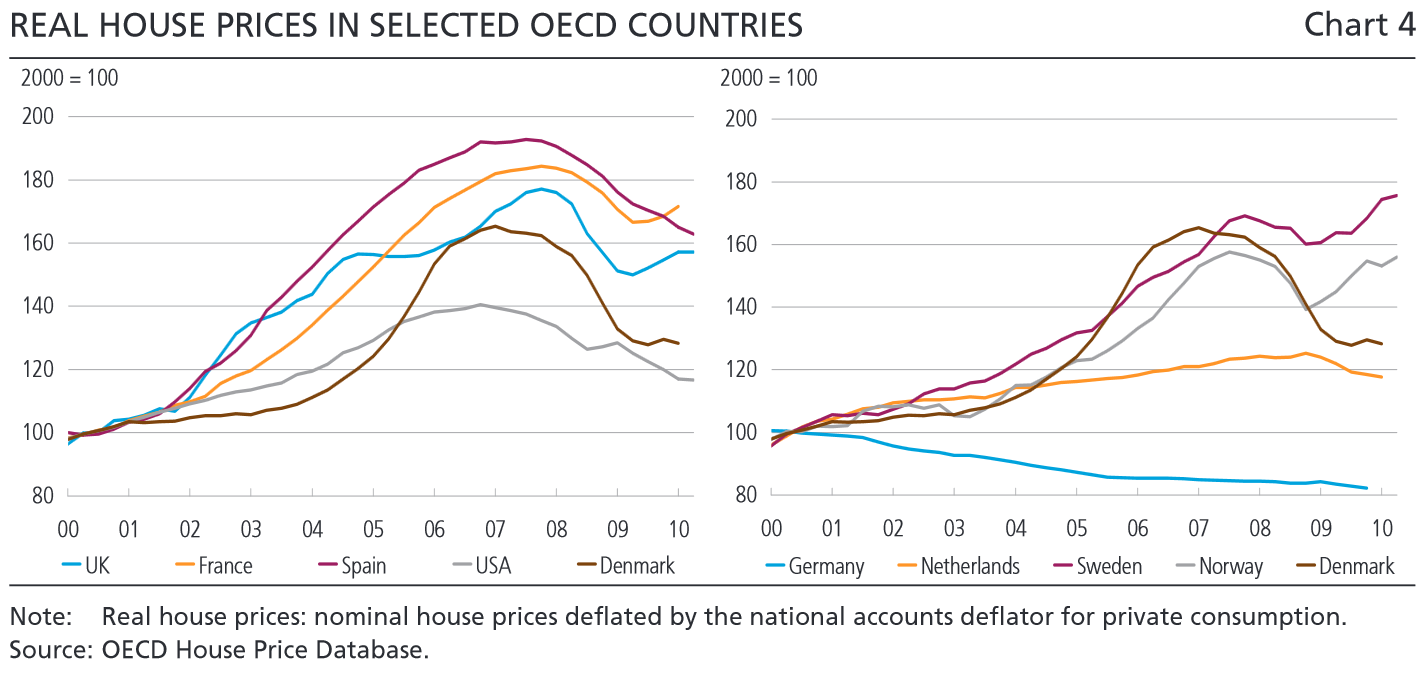
\includegraphics[width=0.9\textwidth]{../figures/intcomparison}
	\centering
	\caption{Taken from \citet[50]{dam2011housing}}\label{dam}
\end{figure}

The second reason we focus on Denmark, is that it is possible to obtain precise and comprehensive data on house price changes, voting returns, and socio-economic controls at a very small geographic level. Existing approaches typically examine house price returns at high levels of aggregation corresponding to either counties or entire states. In contrast, we observe house price changes at the zip code level and voting returns and socio-economic controls at the precinct (i.e., polling place) level. This allows for much more precise measurements of the variables of interest and accordingly less attenuation of observed associations. We elaborate on the specifics of the data in the next section.

Turning to the political context, the government in the entire period we investigate (2005-2015) consisted of two different parties. From 2001 to 2011 the Liberal party was in government along with the Conservative party, and from 2011 till 2015 the Social Democratic party and the Liberal party was in power.\footnote{An additional party, the Socialist party, was in government from 2011 to 2013, however, since this party left government before the election, it is excluded when looking at electoral support for the governing party. To get data on electoral support at the previous election, we also use some data from the 2001 election in which the Social Democratic party and the Liberal party was in power.} This change in party incumbency is useful, since it allows us to distinguish effects on incumbent government support from effects on macropartisanship. 


\section{Data}
The key dependent variable in our study is \textit{percent of votes cast for government parties} in each voting precinct.\footnote{Results are similar for only using the prime minister's party.} Each voting precinct corresponds to a single polling place and is this the smallest unit at which voting returns can be observed. We measure this for all precincts in five elections: 2001, 2005, 2007, 2011 and 2015. A number of precincts are redistricted between each election. This is problematic, as we want to use  the precincts as part of a panel data set. There are two ways to deal with this. We can drop precincts, as their geographical boundaries get altered. This would mean dropping roughly 15 pct. of the data on the dependent variable. The other option is to fix the precincts geographical boundaries at one reference election (i.e. 2015), and then recalculate vote returns in any changed precincts, so they match up with the precincts in the reference election.  As many of the changes in geographical boundaries are minor, we opt to do the latter.\footnote{For details of how returns from the redistricted precincts are calculated, see Søren Risbjerg Thomsen's research note at \texttt{\href{http://bit.ly/205OlPi}{bit.ly/205OlPi}}. We will eventually show results for the other option in an appendix.}. 

The key independent variable is \textit{year-over-year change in local house prices}. We obtain house price data from The Danish Mortgage Banks' Federation (\textit{Realkreditforeningen}), which publishes quarterly data on all house price sales at the zip code level.\footnote{Available at \texttt{\href{http://statistik.realkreditforeningen.dk/}{statistik.realkreditforeningen.dk}}.} Data is presented for houses and apartments separately, so for each zip code we calculate an average of house and apartment price changes weighted by the volume of sales in each category. For each election, we calculate change in house prices as the percentage change in the quarter of the election compared to the same quarter one year before.

In addition to change in house prices, we also calculate a measure of \textit{house price volatility} for each election-year zip code. We calculate volatility as the sales volume-weighted average of the standard deviations of house and apartment price levels over the past eight quarters. In short, the volatility measure captures how much prices change overall in a given election-year zip code. Although large changes in house prices will mechanically translate into higher observed volatility, the absolute year-over-year change is only moderately strongly correlated with volatility ($r=0.22$). This divergence is due to a substantial number of zip codes where house prices fluctuate over time but exhibit little systematic change. We construct the volatility measure to capture precisely this `bubblyness' which characterizes house prices in some localities at some points in time.

As an illustration of the house price volatility measure, consider Figure \ref{volcases}, which plots the highest and lowest levels of observed volatility, respectively Rungsted Kyst (left) and Roslev (right), both in 2007.

\begin{figure}[htbp!]
	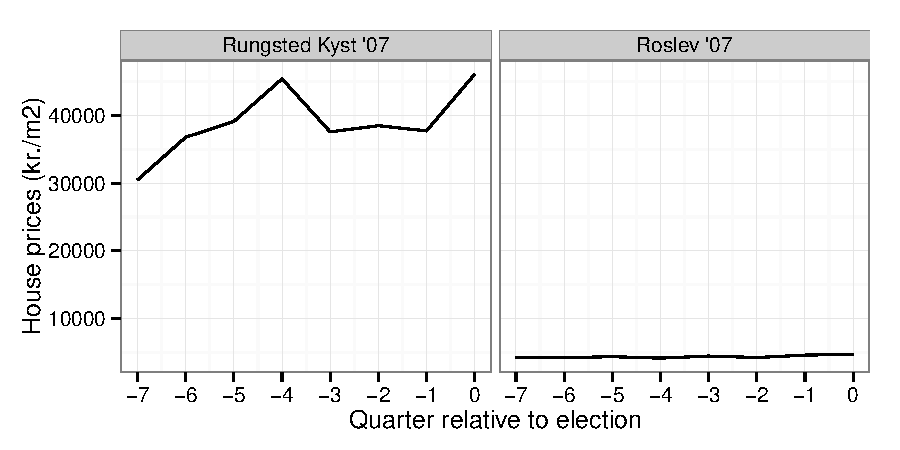
\includegraphics[width=0.9\textwidth]{../figures/volcases}
	\centering
	\caption{Illustration of house price volatility measure: the election year zip codes with the highest and lowest levels of observed volatility, respectively Rungsted Kyst (left) and Roslev (right), both in 2007.}\label{volcases}
\end{figure}

We observe both the change and volatility measures at the zip code level. Since the dependent variable is observed at the voting precinct level, merging these observations is not trivial. The easiest solution would be to extract the zip code of the address of each polling place and link the polling place to house prices in that zip code. Unfortunately, full addresses are not available for all polling places. Instead, we take a three-stage approach to linking polling places to zip codes. First, we extract the street address and higher-level voting district of each polling place and add `Denmark' at the end of the string (the full resulting string is of the format `Streetname X, City, Denmark'). Second, we pass this string to the Google Maps API, which geocodes the string and returns latitude-longitude coordinates.\footnote{Available at \texttt{\href{https://developers.google.com/maps/documentation/geocoding/intro}{developers.google.com/maps/documentation/geocoding/intro}}.} Third and last, we pass these coordinates to the Danish Addresses Web API (DAWA), a public service provided by the Danish Geodata Agency.\footnote{Available at \texttt{\href{http://dawa.aws.dk/}{dawa.aws.dk}}.} The DAWA returns the zip code for each address, allowing us to link the two sources of data. Since voting returns are thus statistically speaking nested inside zip codes, we estimate models using standard errors clustered at the zip code level.

In addition to the main independent variables, we measure a number of structural factors at voting precinct. These are population based measures of economic characteristics of the precincts, which are originally from Statistics Denmark. These are only available at one point in time (2011), and as such cannot be modeled dynamically. The variables are income, average household income in the precinct in DKK, employment, the percentage of people in the precinct who are on the job market, benefits, the percentage of people in the precinct who are on unemployment benefits (`kontanthjælp' and `dagpenge'), and wealth, average household wealth in the precinct in DKK.  


\section{The effect of house prices}

\subsection{Identification strategy}

In this paper we want to identify the causal effect of recent changes in precinct level house prices on electoral support for governing parties. Ideally, we would like to compare support for governing parties in the same district at a specific election across different levels of house-prices. As precincts were only assigned one change in house prices per election, this is obviously not feasible. Instead, we need to construct a feasible observable counterfactual to a precinct with a specific change in house prices, which we can use to difference out the effect of house prices. 

One way to do this, is to simply compare incumbent support at different levels of house price changes across elections and within precincts. Here the counterfactual for any given precinct is the incumbent support of an cross-elections average precinct. A key challenge to causal identification in this case, is that certain structural features of precincts in which house prices are likely to increase might make incumbents more popular. 

We can begin to deal with this problem by examining the historical precinct-specific levels of incumbent support. As such, instead of simply using an average of all precincts as our counterfactual, we can use the average for the individual precinct. Comparing incumbent support within precincts and across different levels of house prices. This takes into account that certain precincts might be historically more inclined to support incumbents and have increasing house prices. However, it does not take into account that when house prices are relatively high in a district in a particular election, it is also likely to be high in other precincts as well. This is problematic if incumbents do systematically better or worse, in general, when house prices are doing well.

To address this problem, we can examine levels of incumbents support, not just relative to the precincts history, but also relative to the level of incumbent support across districts. In this case, our counterfactual for any given precinct is the electoral support, that governing parties typically obtain in that precinct, plus or minus the overall change in electoral support for governing parties across all precincts. This gives us a difference in difference approach to identifying the effect of house prices. As such, we look at differences within elections in differences between the individual precincts typical and actual outcome.

The difference-in-difference approach makes it possible to compare with a very reasonable counterfactual situation - what is the typical incumbent support we could expect in a precinct given the overall popularity of the incumbent. However, since the the governing parties change from election to election, and since the priorities of the same parties might change from election to election, different types of precincts might prefer government parties at  different elections. This poses a challenge to causal identification. As such,  these changes in election and precinct-specific preferences might not be the same across types of precincts which experience increasing and decreasing in house prices. We cannot completely deal with this problem; as mentioned in the beginning of this section we have only one piece of information on the assigned house price change for a precinct at an individual election. However, we can create an even more appropriate counter-factual by taking into account how precincts of a specific type do at specific elections.

First, we can take the precincts economic status into account. That is, how the incumbent scores on the four structural variables mentioned above: income, wealth, employment and benefits. In this case our counterfactual for any precinct will be be the typical incumbent support we would expect a precinct to have given how popular the incumbent is at this specific election in precincts with a similar economic make-up.

Second, we can take the precincts geographical location into account. Specifically, we can look at what municipality,  the smallest local administrative unit in Denmark, the municipality is located in. In this case our counterfactual for any precinct will be be the typical incumbent support we would expect a precinct to have given how popular the incumbent is at this specific election in precincts in the same municipality.

This counter-factual can be expressed using the following linear equation.

\begin{equation}
y_{it}= \delta houseprices_{it} + \pi_i + year_{it} + \epsilon_{it}
\end{equation}

Where $y_{it}$ is incumbent support at election $t$ in precinct $i$ and $houseprices_{it}$ is year-over-year changes in house prices. $\delta$ is the coefficient of interest, as it represents the effect of house prices on incumbent support.  $\pi_i$ represent precinct fixed-effects and $\epsilon_{it}$ is an error term. $year_{it}$ is a year and precinct specific term, which signifies how much more or less popular, we would expect the incumbent to be in an individual precinct at a specific election, given its geographical location and economic status. It is defined as

\begin{equation}
year_{it}=\mathbf{X_i\beta_t + Z_i\gamma_t}
\end{equation}

$ \mathbf{X_i}$ is a vector of the four economic variables and $\mathbf{\beta_t}$ is a vector of coefficients attached to these variables, which specify the relationship between these variables and incumbent popularity at time $t$. $\mathbf{Z_i}$ is a vector of 98 dummy variables indicating which of 98 municipalities the precinct lies within. $\mathbf{\gamma_t}$ is a vector of coefficients attached to these dummy variables, which specify the cross-precinct municipal average of incumbent popularity at time $t$.


\subsection{Estimating the average effect of house prices}
In order to examine the relationship between electoral support for governing parties and local house prices, we estimate a number of different versions of equation (1) in table \ref{tab1}. In model 1 we simply look at the bivariate relationship between electoral support and house prices. In model 2 we include precinct fixed effects. In model 3 we include year fixed effects; this gives us the difference-in difference model. In model 4 we include year by structural factors. In model 5 we include year by municipality fixed effects. The standard errors are robust and clustered at the precinct level.\footnote{Since all precincts are nested within zip-codes, this is more restrictive than zip-code clustering.}

As can be seen from table \ref{tab1}, there is a statistically significant and positive effect estimate of one-year changes in house prices, indicating that a larger fraction of the electorate casts their vote for governing parties in precincts where house prices increase. In the most demanding specification, model 5, the effect is roughly 0.01. this signifies that if house prices increase one percentage points, governing politicians get 0.01 percentage point fewer votes. A small but meaningful average effect.


\begin{table}[htbp]\centering
\def\sym#1{\ifmmode^{#1}\else\(^{#1}\)\fi}
\caption{Estimated effects of house prices on electoral support for governing parties.} \label{tab1}
\begin{tabular}{l*{5}{c}}
\hline\hline
                    &\multicolumn{1}{c}{(1)}        &\multicolumn{1}{c}{(2)}        &\multicolumn{1}{c}{(3)}        &\multicolumn{1}{c}{(4)}        &\multicolumn{1}{c}{(5)}        \\
\hline
$\Delta$ house price&        0.10\sym{**}&        0.12\sym{**}&        0.05\sym{**}&        0.05\sym{**}&        0.01\sym{*} \\
                    &      (0.01)        &      (0.01)        &      (0.01)        &      (0.01)        &      (0.01)        \\
[1em]
\hline Precinct FE  &                    &$\checkmark$        &$\checkmark$        &$\checkmark$        &$\checkmark$        \\
[1em]
Year FE             &                    &                    &$\checkmark$        &$\checkmark$        &$\checkmark$        \\
[1em]
Year FE * Structural factors&                    &                    &                    &$\checkmark$        &$\checkmark$        \\
[1em]
Year FE * Municipality FE&                    &                    &                    &                    &$\checkmark$        \\
\hline
Observations        &        4192        &        4192        &        4192        &        4170        &        4170        \\
RMSE                &        8.40        &        7.16        &        5.71        &        4.77        &        2.84        \\
\hline\hline
\multicolumn{6}{l}{\footnotesize Standard errors in parentheses}\\
\multicolumn{6}{l}{\footnotesize \sym{*} \(p<0.05\), \sym{**} \(p<0.01\)}\\
\end{tabular}
\end{table}


If we have identified a causal effect of house prices in model (1) of table 1, we would not expect there to be any systematic difference in incumbent support over time between those precincts which happen to have increasing house prices at any given election and those who happen to have decreasing house prices at any given election.  In tables \ref{tab2} and \ref{tab3} we try to test this by using a one-period lag and one-period lead of the dependent variable respectively.

\begin{table}[htbp]\centering
\def\sym#1{\ifmmode^{#1}\else\(^{#1}\)\fi}
\caption{Estimated effects of house prices on electoral support for governing parties at t+1.} \label{tab2}
\begin{tabular}{l*{5}{c}}
\hline\hline
                    &\multicolumn{1}{c}{(1)}        &\multicolumn{1}{c}{(2)}        &\multicolumn{1}{c}{(3)}        &\multicolumn{1}{c}{(4)}        &\multicolumn{1}{c}{(5)}        \\
\hline
$\Delta$ house price&        0.12\sym{**}&        0.14\sym{**}&       -0.02        &       -0.01        &        0.02        \\
                    &      (0.01)        &      (0.01)        &      (0.01)        &      (0.01)        &      (0.01)        \\
[1em]
\hline Precinct FE  &                    &$\checkmark$        &$\checkmark$        &$\checkmark$        &$\checkmark$        \\
[1em]
Year FE             &                    &                    &$\checkmark$        &$\checkmark$        &$\checkmark$        \\
[1em]
Year FE * Structural factors&                    &                    &                    &$\checkmark$        &$\checkmark$        \\
[1em]
Year FE * Municiplaity FE&                    &                    &                    &                    &$\checkmark$        \\
\hline
Observations        &        3227        &        3227        &        3227        &        3209        &        3209        \\
RMSE                &        8.62        &        7.11        &        6.22        &        5.24        &        3.05        \\
\hline\hline
\multicolumn{6}{l}{\footnotesize Standard errors in parentheses}\\
\multicolumn{6}{l}{\footnotesize \sym{*} \(p<0.05\), \sym{**} \(p<0.01\)}\\
\end{tabular}
\end{table}


\begin{table}[htbp]\centering
\def\sym#1{\ifmmode^{#1}\else\(^{#1}\)\fi}
\caption{Estimated effects of house prices on electoral support for governing parties at t-1.} \label{tab3}
\begin{tabular}{l*{4}{c}}
\hline\hline
                    &\multicolumn{1}{c}{(1)}        &\multicolumn{1}{c}{(2)}        &\multicolumn{1}{c}{(3)}        &\multicolumn{1}{c}{(4)}        \\
\hline
$\Delta$ house price&       -0.03\sym{**}&       -0.04\sym{**}&        0.07\sym{**}&        0.08\sym{**}\\
                    &      (0.01)        &      (0.01)        &      (0.01)        &      (0.01)        \\
[1em]
\hline Precinct FE  &                    &$\checkmark$        &$\checkmark$        &$\checkmark$        \\
[1em]
Year FE             &                    &                    &$\checkmark$        &$\checkmark$        \\
[1em]
Year FE * Structural factors&                    &                    &                    &$\checkmark$        \\
\hline
Observations        &        4197        &        4197        &        4197        &        4173        \\
RMSE                &        8.80        &        7.50        &        6.46        &        5.04        \\
\hline\hline
\multicolumn{5}{l}{\footnotesize Standard errors in parentheses}\\
\multicolumn{5}{l}{\footnotesize \sym{*} \(p<0.05\), \sym{**} \(p<0.01\)}\\
\end{tabular}
\end{table}



As can be seen from the tables \ref{tab2} and \ref{tab3} neither the lead nor the lag dependent variable models show a significant  effect of house prices in the most demanding models. This suggests that the effect identified above is in fact causal.



\subsection{Heterogeneity}

We examine two different sources of heterogeneity in the effect of house prices. Analyzing heterogeneity in the effect is important as it help us understand the implications  of the effect for reelection-minded governing politicians. Specifically, it tells us whether politicians have a interest in promoting or avoiding  specific types of house-price changes in designing economic policy with implications for the housing market. %However, it is also somewhat dangerous as issues of multiple comparisons and over-fitting becomes prevalent. To avoid this we limit our selfs to examining types of heterogeneity, which are firmly based on previous literature on economic voting.

The first source of heterogeneity is the sign of the changes in house prices. A small literature in economic voting have identified a negativity bias in economic voting, in that voters react more strongly to negative economic outcomes, than they do to positive economic outcomes \citep[e.g.][]{bloom1975voter}. In order to investigate whether a similar negativity bias is present in our dataset, we decompose our house price variable into two different variables. A variable which records positive changes in house prices, and which is zero if the changes are negative, and a variable which records negative changes in house prices (numerically), and which is zero if changes in house prices are positive. In table \ref{tab4} we estimate the same models as above, but with our new positive and negative house price change variables. We also include a statistical test of whether the effect of the two variables are numerically similar. 

As can be seen from table \ref{tab4} the negative changes have a significantly larger effect than the positve changes in the most demanding specification (model 4). This indicates that there is a negativity bias in the effect of house prices; negative changes are more likely to affect election results than positive changes. 

\begin{table}[htbp]\centering
\def\sym#1{\ifmmode^{#1}\else\(^{#1}\)\fi}
\caption{Estimated effects of house prices on electoral support for governing parties across positive and negative changes.} \label{tab4}
\begin{tabular}{l*{4}{c}}
\hline\hline
                    &\multicolumn{1}{c}{(1)}         &\multicolumn{1}{c}{(2)}         &\multicolumn{1}{c}{(3)}         &\multicolumn{1}{c}{(4)}         \\
\hline
$\Delta$ house price (negative)&       -0.08\sym{***}&       -0.11\sym{***}&       -0.07\sym{***}&       -0.10\sym{***}\\
                    &      (0.02)         &      (0.03)         &      (0.02)         &      (0.02)         \\
[1em]
$\Delta$ house price (positive)&        0.12\sym{***}&        0.12\sym{***}&        0.04\sym{***}&        0.04\sym{**} \\
                    &      (0.01)         &      (0.02)         &      (0.01)         &      (0.01)         \\
[1em]
\hline Precinct  FE &                     &$\checkmark$         &$\checkmark$         &$\checkmark$         \\
[1em]
Year FE             &                     &                     &$\checkmark$         &$\checkmark$         \\
[1em]
Year FE * Structural factors&                     &                     &                     &$\checkmark$         \\
\hline
Test of no difference (p)&        0.26         &        0.84         &        0.24         &        0.02         \\
Observations        &        4192         &        4192         &        4192         &        4170         \\
RMSE                &        8.41         &        7.16         &        5.71         &        4.77         \\
\hline\hline
\multicolumn{5}{l}{\footnotesize Standard errors in parentheses}\\
\multicolumn{5}{l}{\footnotesize \sym{*} \(p<0.05\), \sym{**} \(p<0.01\), \sym{***} \(p<0.001\)}\\
\end{tabular}
\end{table}


This asymmetric effect is plotted in figure \ref{posneg}.

\begin{figure}[htbp]
	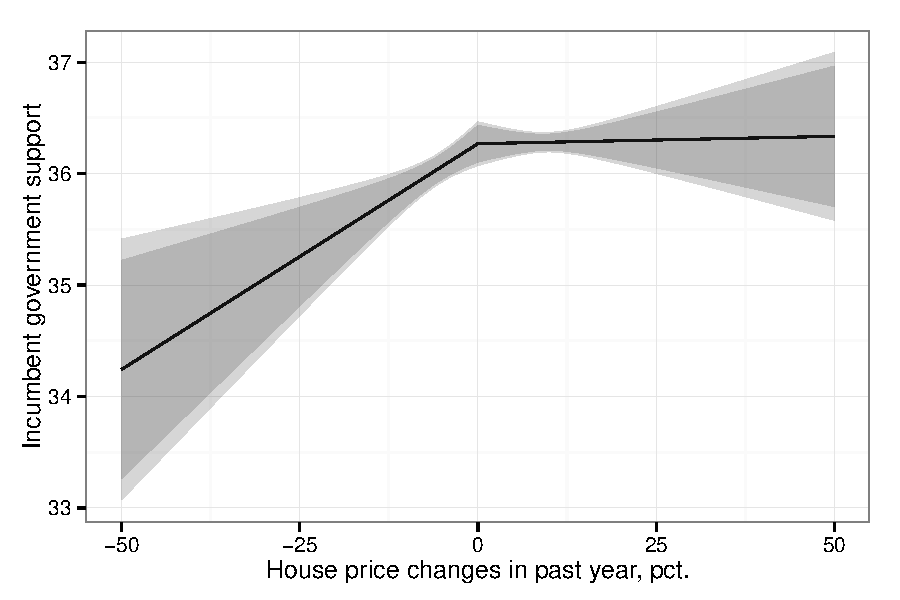
\includegraphics[page=1,width=0.8\textwidth]{../figures/posnegplot}
	\centering
	\caption{Predicted electoral support for governing parties across changes in house prices with 90 and 95 pct. confidence intervals. Derived from model (4) in table \ref{tab4}}
	\label{posneg}
\end{figure}

The second source of heterogeneity is volatility in house prices. In table \ref{tab5} we look at differences in the effect of changes in house prices across different levels of volatility in the house prices.  We do this by extending the models estimated above with an interaction between the house price variable and our volatility variable. The interaction is statistically significant in the two most demanding specifications (models 3 and 4). This suggests, that house prices have a greater impact on election results in areas were house prices are generally more volatile. 

\begin{table}[htbp]\centering
\def\sym#1{\ifmmode^{#1}\else\(^{#1}\)\fi}
\caption{Estimated effects of house prices on electoral support for governing parties across volatility.} \label{tab5}
\begin{tabular}{l*{4}{c}}
\hline\hline
                    &\multicolumn{1}{c}{(1)}        &\multicolumn{1}{c}{(2)}        &\multicolumn{1}{c}{(3)}        &\multicolumn{1}{c}{(4)}        \\
\hline
$\Delta$ housing price&       -0.01        &       -0.20\sym{**}&       -0.18\sym{**}&       -0.17\sym{**}\\
                    &      (0.03)        &      (0.02)        &      (0.02)        &      (0.03)        \\
[1em]
Log(density)        &       -5.49\sym{**}&       -2.69\sym{**}&        0.00        &        0.00        \\
                    &      (0.37)        &      (0.41)        &         (.)        &         (.)        \\
[1em]
$\Delta$ housing price $\times$ Log(density)&        0.05\sym{**}&        0.12\sym{**}&        0.10\sym{**}&        0.10\sym{**}\\
                    &      (0.01)        &      (0.01)        &      (0.01)        &      (0.01)        \\
[1em]
\hline Precinct FE  &                    &                    &$\checkmark$        &$\checkmark$        \\
[1em]
Year FE             &                    &                    &                    &$\checkmark$        \\
\hline
Observations        &        4193        &        4173        &        4173        &        4173        \\
RMSE                &        8.42        &        6.80        &        5.50        &        5.40        \\
\hline\hline
\multicolumn{5}{l}{\footnotesize Standard errors in parentheses}\\
\multicolumn{5}{l}{\footnotesize \sym{*} \(p<0.05\), \sym{**} \(p<0.01\)}\\
\end{tabular}
\end{table}


This interaction effect is plotted in figure \ref{vola}.

\begin{figure}[htbp]
	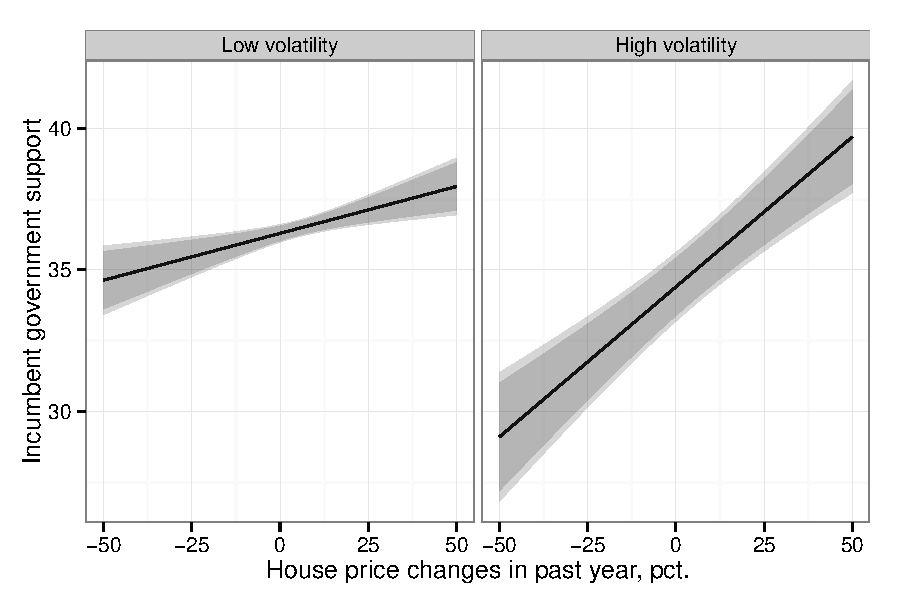
\includegraphics[page=1,width=0.8\textwidth]{../figures/volaplot}
	\centering
	\caption{Predicted electoral support for governing parties across changes in house prices at the 5th and 95th percentile of the volatility variable with 90 and 95 pct. confidence intervals. Derived from model (4) in table \ref{tab5}}
	\label{vola}
\end{figure}


In table \ref{tab6} and figure \ref{volaposneg} we look at the relationship between both types of heterogeneity. The picture which emerges is one where house prices are very important for the succes of incumbent government parties if house prices decrease in more volatile areas, however, if they increase or if the changes happen in less volatile areas, they are less important.

\begin{table}[htbp]\centering
\def\sym#1{\ifmmode^{#1}\else\(^{#1}\)\fi}
\caption{Estimated effects of house prices on electoral support for governing parties across volatility.} \label{tab6}
\begin{tabular}{l*{5}{c}}
\hline\hline
                    &\multicolumn{1}{c}{(1)}        &\multicolumn{1}{c}{(2)}        &\multicolumn{1}{c}{(3)}        &\multicolumn{1}{c}{(4)}        &\multicolumn{1}{c}{(5)}        \\
\hline
$\Delta$ house price (positive)&        0.15\sym{**}&        0.11\sym{**}&        0.02        &        0.03        &       -0.04\sym{*} \\
                    &      (0.03)        &      (0.04)        &      (0.03)        &      (0.02)        &      (0.02)        \\
[1em]
$\Delta$ house price (negative)&       -0.05        &       -0.16\sym{*} &        0.03        &        0.02        &       -0.07\sym{*} \\
                    &      (0.07)        &      (0.06)        &      (0.05)        &      (0.05)        &      (0.03)        \\
[1em]
Volatility          &       -7.22        &        0.14        &        7.29\sym{**}&       -1.16        &       -1.73        \\
                    &      (3.72)        &      (3.25)        &      (2.70)        &      (2.03)        &      (1.60)        \\
[1em]
$\Delta$ house price (positive) $\times$ Volatility&       -0.10        &        0.04        &        0.05        &        0.03        &        0.19\sym{**}\\
                    &      (0.12)        &      (0.13)        &      (0.09)        &      (0.07)        &      (0.06)        \\
[1em]
$\Delta$ house price (negative) $\times$ Volatility&       -0.01        &        0.19        &       -0.54\sym{**}&       -0.50\sym{**}&        0.12        \\
                    &      (0.28)        &      (0.24)        &      (0.21)        &      (0.17)        &      (0.12)        \\
[1em]
\hline Precinct FE  &                    &$\checkmark$        &$\checkmark$        &$\checkmark$        &$\checkmark$        \\
[1em]
Year FE             &                    &                    &$\checkmark$        &$\checkmark$        &$\checkmark$        \\
[1em]
Year FE * Structural factors&                    &                    &                    &$\checkmark$        &$\checkmark$        \\
[1em]
Year FE * Municipality FE&                    &                    &                    &                    &$\checkmark$        \\
\hline
Observations        &        4184        &        4184        &        4184        &        4162        &        4162        \\
RMSE                &        8.46        &        7.17        &        5.70        &        4.76        &        2.84        \\
\hline\hline
\multicolumn{6}{l}{\footnotesize Standard errors in parentheses}\\
\multicolumn{6}{l}{\footnotesize \sym{*} \(p<0.05\), \sym{**} \(p<0.01\)}\\
\end{tabular}
\end{table}


\begin{figure}[htbp]
	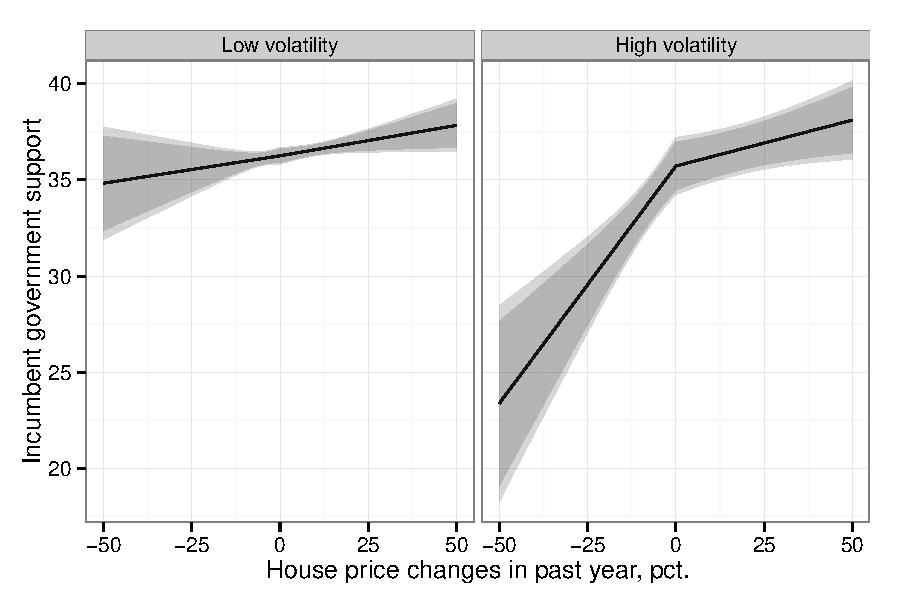
\includegraphics[width=0.8\textwidth]{../figures/volaposnegplot}
	\centering
	\caption{Predicted electoral support for governing parties across changes in house prices at the 5th and 95th percentile of the volatility variable with 90 and 95 pct. confidence intervals. Derived from model (4) in table \ref{tab6}}
	\label{volaposneg}
\end{figure}




\section{Conclusion}
Short summary

Implications for policy-makers

Shortcomings




%Appendikser
%Overvej et om forhold mellem volatilitet og prisændringer
%Overvej et på et andet kontekstuelt niveau - e.g. kommuner - jf. MAUP.
%Overvej et om robusthed af interaktionsled - evt. lav kommuneinteraktioner, og se om effekten stadig holder
%Overvej det samme som sidste om positiv-negativ
%Overvej om vi skal lave et datasæt med "stabile valgsteder" 
%Overvej om vi får samme resultater med statsministerpartiet.





\clearpage

\singlespacing

\bibliographystyle{apa}
\bibliography{library}

\end{document}
